\documentclass[9pt]{beamer}

%!TEX root = ../notas_de_clase.tex

%preamble

%language
\usepackage[spanish,es-nodecimaldot]{babel}
\usepackage[utf8]{inputenc}
\usepackage{apacite}
\usepackage[absolute,overlay]{textpos}

%packages
\usepackage[Algoritmo]{algorithm}
\usepackage{algorithmicx}
\usepackage[noend]{algpseudocode}
\usepackage{mathtools}
\setlength {\marginparwidth}{2cm}
\usepackage{todonotes}
\usepackage{amsbsy}
\usepackage{amssymb}
\usepackage{amsmath,bm}
\usepackage{dsfont}

\usepackage{xcolor}
\providecommand{\sred}[1]{\textcolor{red}{#1}}
\providecommand{\sblue}[1]{\textcolor{blue}{#1}}
\providecommand{\red}[1]{\textcolor{red}{\text{#1}}}
\providecommand{\blue}[1]{\textcolor{blue}{\text{#1}}}
\providecommand{\redb}[1]{\textcolor{red}{\textbf{#1}}}
\providecommand{\blueb}[1]{\textcolor{blue}{\textbf{#1}}}
\usepackage{graphicx}
\usepackage{fancybox}
\usepackage{booktabs}
\usepackage{caption}
\usepackage{float}
%\usepackage[longend,ruled,algochapter,linesnumbered,lined,boxed,commentsnumbered,spanish]{algorithm2e}
%\usepackage[algo2e]{algorithm2e}
\usepackage{amssymb}
\usepackage{amstext}
\usepackage{bm}
\usepackage{wrapfig}
\usepackage{subcaption} % para_unsupervised_chapter

%formatting

\usepackage[export]{adjustbox}

%caption para figuras
\captionsetup[figure]{width=.8\linewidth, font=small,labelfont={bf},name={Fig.},labelsep=period}
\captionsetup[table]{width=.8\linewidth,font=small,labelfont={bf},name={Tabla},labelsep=period}



\ifx\byn\undefined
    \definecolor{my_blue}{HTML}{C2D5FF}
    \definecolor{my_red}{HTML}{FFC2C2}
    \definecolor{my_yellow}{HTML}{FFFFE0}
\else
    \definecolor{my_blue}{HTML}{FFFFFF}
    \definecolor{my_red}{HTML}{FFFFFF}
    \definecolor{my_yellow}{HTML}{FFFFFF}
\fi


\usepackage[framemethod=TikZ]{mdframed}
\mdfdefinestyle{discusion}{%
    %linecolor=black,
    %outerlinewidth=0pt,
    roundcorner=0pt,
    innertopmargin=5pt,
    innerbottommargin=5pt,
    innerrightmargin=20pt,
    innerleftmargin=20pt,
    backgroundcolor=my_blue}

\colorlet{Green}{green!90}


\mdfdefinestyle{ejemplo}{%
    %linecolor=black,
    %outerlinewidth=0pt,
    roundcorner=0pt,
    innertopmargin=5pt,
    innerbottommargin=5pt,
    innerrightmargin=20pt,
    innerleftmargin=20pt,
    backgroundcolor=my_yellow}


\mdfdefinestyle{pendiente}{%
    style = discusion, 
    backgroundcolor=my_red}


\RequirePackage{url}



%definitions
\def\td{{\text d}}
\def\cN{{\mathcal N}}
\def\cX{{\mathcal X}} 
\def\cC{{\mathcal C}} 
\def\N{{\mathbb N}}
\def\d{{\text d}}
\def\datos{{\mathcal D}}
\def\eye{{\mathbb I}}
\def\ssum{{\scriptstyle\sum}}
\def\bepsilon{{\bm \epsilon}}
\def\tx{\tilde{x}}
\def\tX{\tilde{X}}
\def\thetaMAP{\theta_\text{MAP}}
\newcommand{\gp}{\ensuremath{\mathcal{GP}}}
\newcommand{\pr}{\ensuremath{\mathbb{P}}}
\newcommand{\x}{\ensuremath{\mathbf{x}}}
\newcommand{\z}{\ensuremath{\mathbf{z}}}
\newcommand{\cvector}{\ensuremath{\mathbf{c}}}
\newcommand{\e}{\ensuremath{\mathbf{e}}}
\newcommand{\y}{\ensuremath{\mathbf{y}}}
\newcommand{\bx}{\ensuremath{\textcolor{blue}{X}}}
\newcommand{\by}{\ensuremath{\textcolor{blue}{Y}}}
\newcommand{\rx}{\ensuremath{\textcolor{red}{X_*}}}

\newcommand{\R}{\mathbb{R}}
\newcommand{\norm}[1]{\left\lVert#1\right\rVert}




\DeclareMathOperator*{\argmax}{arg\,max}
\DeclareMathOperator*{\argmin}{arg\,min}
\DeclareMathOperator{\E}{\mathbb{E}}
\DeclareMathOperator{\V}{\mathbb{V}}
\DeclareMathOperator{\KL}{\text{KL}}
\DeclareMathOperator{\MVN}{\text{MVN}}
\newcommand\deq{\stackrel{\mathclap{\normalfont\mbox{\tiny def}}}{=}}
%\newcommand{\E}[1]{\mathbb E \left[#1\right]}
\newcommand{\trace}[1]{\text{Tr} \left[#1\right]}


\usepackage{amsthm}

%-------------------------------------------
% Newtheorem
%-------------------------------------------
\newtheorem{axioma}{\textcolor{red}{Axioma}}
\newtheorem{definicion}{Definición}
\newtheorem*{notacion}{Notación}
\newtheorem{teorema}{Teorema}
\newtheorem{corolario}{Corolario}
\newtheorem{lema}{Lema}
\newtheorem{lemaZ}{\textcolor{red}{Lema}}
\newtheorem{propiedad}{Propiedad:}
\newtheorem{proposicion}{Proposición:}
\newtheorem*{observacion}{Observación}
\newtheorem*{comentario}{Comentario}
\newtheorem*{ejemplo}{Ejemplo}
\newtheorem*{resultado}{Resultado}
\newtheorem*{propuesto}{Ejercicio propuesto}
\newtheorem*{demostracion}{Demostración} % No se usa, usar \begin{proof}\end{proof} que son por default.

%listing paackage para código
\usepackage{listings}
\usepackage{xcolor}
 
\definecolor{codegreen}{rgb}{0,0.6,0}
\definecolor{codegray}{rgb}{0.5,0.5,0.5}
\definecolor{codepurple}{rgb}{0.58,0,0.82}
\definecolor{backcolour}{rgb}{0.95,0.95,0.92}
 
\lstdefinestyle{mystyle}{
    xleftmargin=0.15\textwidth,
    linewidth=0.8\textwidth,
    backgroundcolor=\color{backcolour},   
    commentstyle=\color{codegreen},
    keywordstyle=\color{magenta},
    numberstyle=\tiny\color{codegray},
    stringstyle=\color{codepurple},
    basicstyle=\ttfamily\footnotesize,
    breakatwhitespace=true,         
    breaklines=true,                 
    captionpos=b,                    
    keepspaces=true,                 
    numbers=left,                    
    numbersep=5pt,                  
    showspaces=false,                
    showstringspaces=false,
    showtabs=false,                  
    tabsize=2
}
 
\lstset{style=mystyle}

\numberwithin{equation}{section}

\usetheme{simple}

\title{Clase 20 - Procesos Gaussianos I}
\subtitle{Aprendizaje de Máquinas - MA5204}
\date{\today}
\author{Felipe Tobar} 
\titlegraphic{
\begin{figure}[htp] 
    \centering
        
\includegraphics[width=0.15\textwidth]{../img/Uchile.pdf}% 
\end{figure}
}
\institute{Department of Mathematical Engineering \&\\ Center for Mathematical Modelling\\Universidad de Chile}

\begin{document}
\begin{frame}
  \titlepage
\end{frame}

\section{Procesos Gaussianos}

\begin{frame}{Modelos paramétricos y no paramétricos}
\begin{itemize}
  \item \textbf{Modelos paramétricos: } Son los modelos que hemos considerado hasta ahora y que se caracterizan por su cantidad fija de parámetros al momento de entrenar. \\ \pause 
  Ejemplo: Regresión lineal/no lineal \pause 
  \item \textbf{Modelos no paramétricos: } Son los modelos que no tienen un número fijo de parámetros, pudiendo llegar incluso a ser infinitos. \\ \pause 
  Ejemplo: Máquinas de soporte vectorial. \pause 

\end{itemize}

\begin{observacion}
Es importante hacer la distinción entre parámetros que se aprenden y los parámetros del modelo (hiperparámetros), donde estos últimos pueden ser fijos independiente de si el método es paramétrico o no paramétrico.
\end{observacion} \pause 

En este capítulo introduciremos un método no paramétrico probabilístico de regresión no lineal, llamado procesos gaussianos ($\gp$). Este modelo en vez de encontrar un candidato único de la función a estimar, define una distribución sobre funciones $\mathbb{P}(f)$, donde $f$ es una función de un espacio de entrada $\mathcal{X}$ a los reales, $f: \mathcal{X} \rightarrow \mathbb{R}$. Esto tiene la virtud de permitir cuantificar la incertidumbre puntual que existe en la predicción de nuestro modelo, la cual servirá en forma de intervalos de confianza para la distribución gaussiana.

\end{frame}

\begin{frame}{Proceso Gaussiano}

\begin{definition}[proceso gaussiano]
  Un proceso gaussiano ($\gp$) es una colección de variables aleatorias, tal que para cualquier subconjunto finito de puntos, estos tienen una distribución conjuntamente gaussiana.
\end{definition} \pause

Al aplicar esta definición a nuestro caso anterior, $\pr(f)$ será un $\gp$ y para cualquier conjunto finito $\{ x_i\}_{i=1}^{n}  \subset \mathcal{X}$, la distribución de $\pr(f(\mathbf{x}))$ es Gaussiana multivariada $f(\mathbf{x})=(f(x_1), \ldots, f(x_n))^\top$). En este caso las variables aleatorias representan el valor de la función $f(x_i)$ en la posición $x_i$. \pause
\vspace{0.2cm}

Un $\gp$ queda completamente caracterizado por su función de media $m(\cdot)$ y función de covarianza $K(\cdot, \cdot)$, de esta forma para cualquier conjunto finito podemos encontrar la distribución. Definimos estas funciones como
\begin{align*}
  m(x) & = \mathbb{E}\left\{f(x)\right\}\\
  K(x, x') & = \mathbb{E}\left\{\left(f(x) - m(x)\right) \left(f(x') - m(x') \right)\right\}
\end{align*}


\end{frame}

\begin{frame}{Proceso Gaussiano}

Y de esta forma podemos escribir el proceso como: \pause 

\begin{equation*}
  f \sim \gp(m(\cdot), K(\cdot, \cdot))
\end{equation*}  \pause 

Donde para un conjunto finito tenemos que la marginal resulta de la forma:
\pause
\begin{equation*}
  f(\x) \sim \mathcal{N}(m(\x), K(\x, \x))
\end{equation*} \pause 



Hasta el momento hemos hablado del espacio de entrada $\mathcal{X}$ como genérico, un caso común es definir los $\gp$ sobre el tiempo ($\mathbb{R}^{+}$), es decir que los $x_i$ son instantes de tiempo. Es de notar que este no es el único caso, y se podría definir sobre un espacio más general, por ejemplo $\mathbb{R}^d$. \pause

\vspace{0.2cm}

Otro punto a notar es que como estamos hablando de una colección (no necesariamente finita) de variables aleatorias, es necesario que se cumpla la propiedad de marginalización (o llamada consistencia). Esta propiedad se refiere a que si un $\gp$ define una distribución multivariada para digamos dos variables $(y_1, y_2) \sim \mathcal{N}(\mu, \Sigma)$ entonces también debe definir $y_1 \sim \mathcal{N}(\mu_1, \Sigma_{11})$ donde $\mu_1$ es la componente respectiva del vector $\mu$ y $\Sigma_{11}$ la submatriz correspondiente de $\Sigma$. En otras palabras, el tomar un subconjunto más grande de puntos no cambia la distribución de un subconjunto más pequeño. Y podemos notar que esta condición se cumple si tomamos la función de covarianza definida anteriormente.

\end{frame}

\begin{frame}{Muestreo de un GP}

Un $\gp$ define un \textit{prior} sobre funciones, por lo que, antes de ver ningún dato se podría obtener una muestra de este proceso dada una función de media y covarianza. \pause

\vspace{0.2cm}

Consideremos $m(\cdot) = 0$ y función de covarianza (kernel) exponencial cuadrática (o RBF) definida como \pause
\begin{equation*}
  K_{SE}(x, x') = \sigma^2 \exp\left( - \frac{\left( x- x'\right)^2}{2\ell^2} \right)
\end{equation*} \pause

Donde en este caso los parámetros son interpretables (y como veremos más adelante pueden ser aprendidos a través de un conjunto de entrenamiento) donde $\sigma^2$ es la varianza de la función, notar que esta es la diagonal de la matriz covarianza. El parámetro $\ell$ es conocido como el \textit{lenghtscale} que determina que tan lejos tiene influencia un punto sobre otro, donde en general un punto no tendrá influencia más allá de $\ell$ unidades alrededor.

\vspace{0.2cm}

A continuación se presenta un muestreo de un $gp$ con las características anteriores


\end{frame}

\begin{frame}{Muestreo de un GP}

\begin{figure}[H]
  \centering
  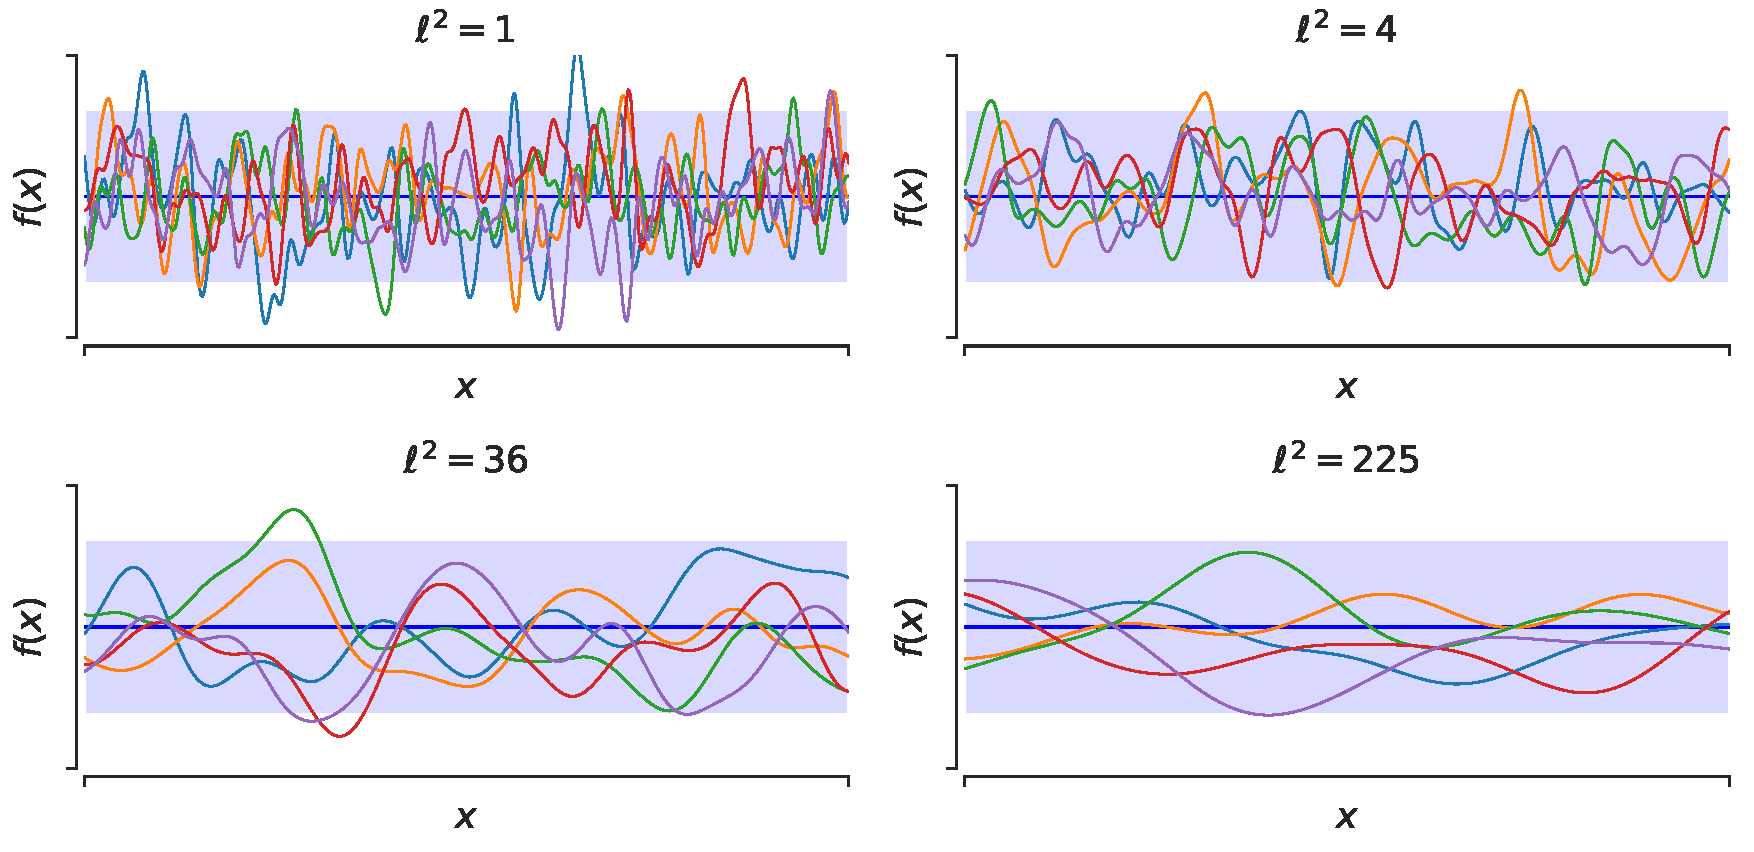
\includegraphics[width=0.9\textwidth]{../img/cap8_prior_muestras}
  \caption{Muestras de un prior $\gp$ con kernel SE, para distintos \textit{lenghtscales} ($\ell$) y función media $m(\cdot)=0$, la parte sombreada corresponde al intervalo de confianza del $95\%$. Se puede ver que a mayor $\ell$ las funciones se van volviendo más suaves.}
  \label{fig:gp_1}
\end{figure}


\end{frame}

\begin{frame}{Incorporando información - Evaluación sin ruido}

Consideremos las observaciones sin ruido de la forma $\{(x_i, f(x_i))\}_{i=1}^{n}$ (conocemos el valor real en $X = [x_1 , \dots , x_n])$. Digamos que queremos realizar una predicción en el conjunto $X_*$ de $n_*$ puntos, luego la distribución conjunta es de la forma: \pause 

\begin{align*}
  \begin{bmatrix} f(X) \\ f(X_*)  \end{bmatrix}
  \sim \mathcal{N} \left(
  \begin{bmatrix} m(X) \\ m(X_*)  \end{bmatrix}, 
  \begin{bmatrix}
    K(X, X) & K(X, X_*) \\ K(X_*, X) & K(X_*, X_*)
  \end{bmatrix}
   \right)
\end{align*} \pause 

El punto clave para realizar predicciones, es el siguiente lema \pause 

\begin{lemma}
  Dado un prior $\gp$ sobre $f(\cdot)$ y una verosimilitud Gaussiana, la posterior sobre $f(\cdot)$ es también un $\gp$. Además, se puede condicionar sobre las observaciones $(X, f(X))$ para obtener

\begin{equation*}
  f(X_*)|f(X), X  \sim \mathcal{N}(m_{X_*|X}, \Sigma_{X_*|X}) \label{eq:gp_post}
\end{equation*}

Donde la media y covarianza son:
\begin{align*}
  m_{X_*|X} & = m(X_*) + K(X_*, X)K^{-1}(X, X) (f(X) - m(X))\\
   \Sigma_{X_*|X} & = K(X_*, X_*) - K(X_*, X)K^{-1}(X, X) K(X, X_*)
\end{align*}
\end{lemma}

\end{frame}

\begin{frame}{Incorporando información - Evaluación sin ruido}
\begin{figure}[H]
  \centering
  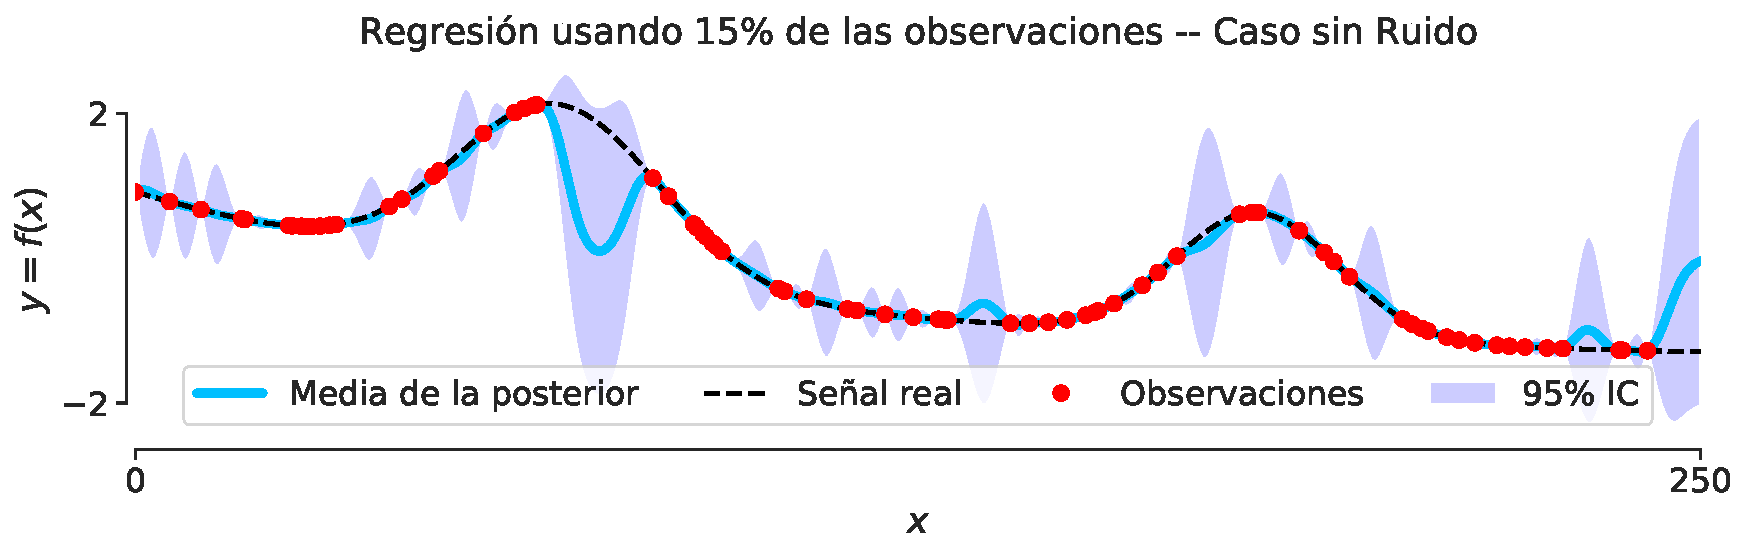
\includegraphics[width=0.9\textwidth]{../img/cap8_posterior_no_ruido}
  \caption{Regresión con $\gp$ para señal sintetica usando el 15$\%$ de los datos muestreados de forma no uniforme, utilizand un $\gp$ de media nula y kernel SE.} 
  \label{fig:gp_2}
\end{figure}


\end{frame}

\begin{frame}{Incorporando información - Evaluación con ruido}

En este caso las observaciones son de la forma $y_i = f(x_i) + \eta$ donde $\eta \sim \mathcal{N}(0, \sigma_n^2)$ por lo que ahora nuestro conjunto de observaciones es de la forma $(X,Y)$ donde $Y=f(X) + \eta$. \\\pause 
Lo que en nuestro modelo equivale a agregar un término a la función de covarianza 

\begin{equation*}
  cov(Y) = K(X, X) + \sigma_n^2\eye
\end{equation*} \pause 

Donde si tenemos el mismo caso anterior, observaciones $(X,Y)$ y queremos evaluar en $X_*$, la conjunta queda \pause 
\begin{align*}
  \begin{bmatrix} Y \\ f(X_*)  \end{bmatrix}
  \sim \mathcal{N} \left(
  \begin{bmatrix} m(X) \\ m(X_*)  \end{bmatrix}, 
  \begin{bmatrix}
    K(X,X) + \sigma_n^2 \eye & K(X, X_*) \\ K(X_*,X) & K(X_*,X_*)
  \end{bmatrix}
   \right)
\end{align*}

\begin{observacion}
Notemos que el termino de ruido solo es agregado al subbloque correspondiente a las observaciones, no se agrega el termino en los otros subbloques pues buscamos hacer una predicción de la función latente $f(\cdot)$ y no una versión ruidosa de esta.
\end{observacion}

\end{frame}

\begin{frame}{Incorporando información - Evaluación con ruido}
Igual que en el caso sin ruido, podemos condicionar esta conjunta a las observaciones y obtenemos el siguiente resultado: \pause


\begin{lemma}
  Para una evaluación con ruido se tiene que
  
  \begin{equation}
    f(X_*)|Y, X  \sim \mathcal{N}(m_{X_*|X}, \Sigma_{X_*|X})\label{eq:gp_posterior}
  \end{equation}
  Donde la media y covarianza son:
  \begin{align}
    m_{X_*|X} & = m(X_*) + K(X_*, X) [K(X, X) + \sigma_n^2 \eye]^{-1} (Y - m(X))\\
   \Sigma_{X_*|X} & = K(X_*, X_*) - K(X_*, X) [K(X, X) + \sigma_n^2 \eye]^{-1} K(X, X_*)
  \end{align}
\end{lemma}


 \end{frame}

 \begin{frame}{Incorporando información - Evaluación con ruido}
 \begin{figure}[H]
  \centering
  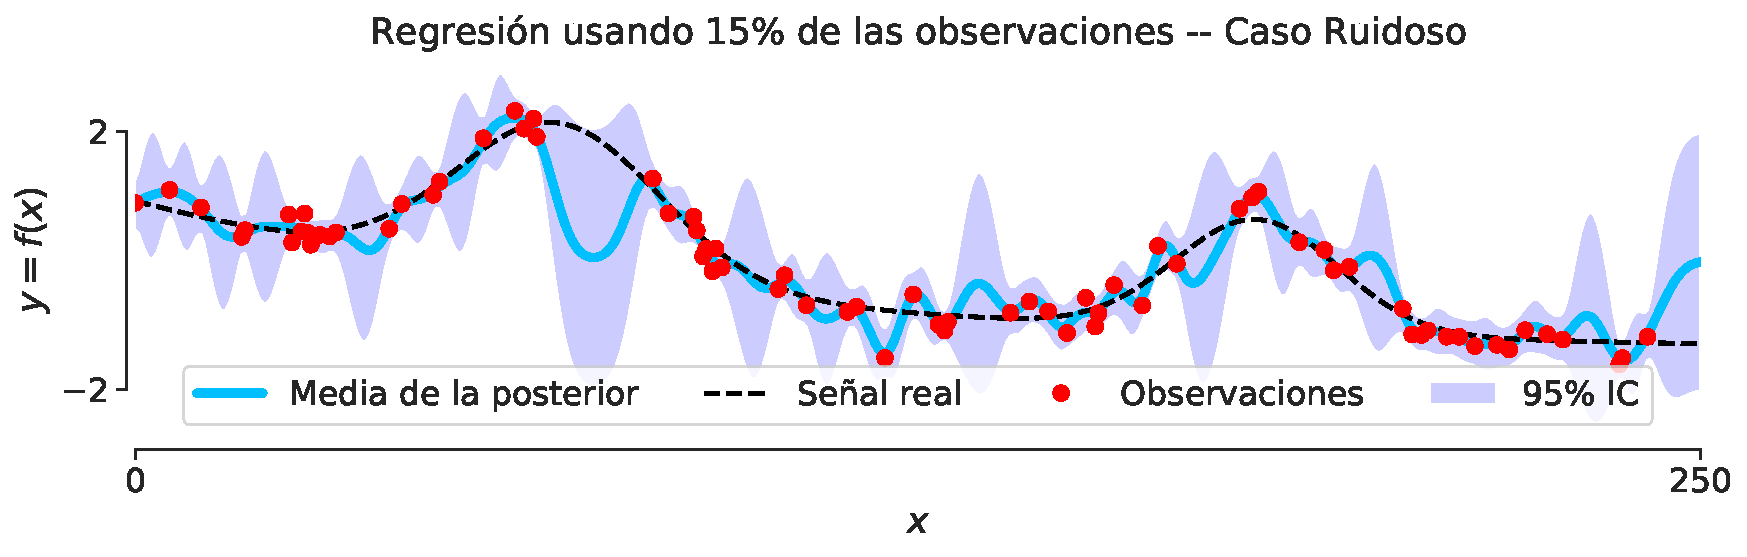
\includegraphics[width=0.9\textwidth]{../img/cap8_posterior_ruido}
  \caption{Regresión con $\gp$ para señal sintetica usando el 15$\%$ de los datos muestreados de forma no uniforme y contaminados con ruido Gaussiano, utilizando un $\gp$ de media nula y kernel SE.}
  \label{fig:gp_3}
\end{figure}

 \end{frame}



\begin{frame}
  \titlepage
\end{frame}




%Quitar de comentarios apenas se agregue alguna referencia 
%\bibliography{../capitulos/referencias} %Bibliografía
%\bibliographystyle{apacite}
\end{document} 